\documentclass[tikz,border=12pt]{standalone}
\usepackage[T1]{fontenc}
\usepackage{mathpazo}
\usepackage{amsmath,amssymb}
\usetikzlibrary{arrows.meta, calc}

\definecolor{stblue}{HTML}{7B97AD}
\definecolor{rwgold}{HTML}{B8995E}
\definecolor{sage}{HTML}{7A9A7E}
\definecolor{dkbrown}{HTML}{3D3530}
\definecolor{wmgray}{HTML}{7B7067}
\definecolor{cream}{HTML}{F9F6F0}
\definecolor{border}{HTML}{D4C9B8}
\definecolor{terracotta}{HTML}{C47A6A}
\definecolor{lavender}{HTML}{907EA0}

\begin{document}
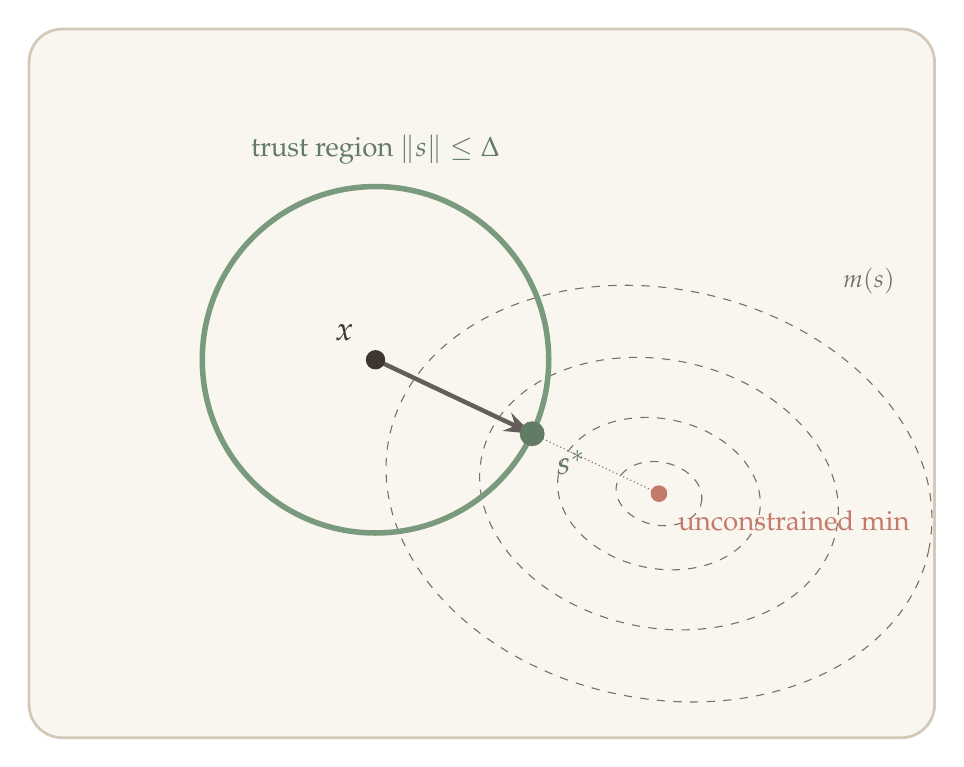
\begin{tikzpicture}[
  >={Stealth[length=3.5mm, width=2.5mm]},
  line width=1.2pt
]

% Background
\fill[cream, rounded corners=12pt] (-5,-4.5) rectangle (6.5,4.5);
\draw[border, line width=1pt, rounded corners=12pt] (-5,-4.5) rectangle (6.5,4.5);

% ── Coordinates ──
% Current point x shifted left so figure is better centered
\coordinate (x) at (-0.6,0.3);
% Unconstrained minimizer of the quadratic model (outside trust region)
\coordinate (umin) at (3.0,-1.4);
% Trust region radius
\pgfmathsetmacro{\trradius}{2.2}
% Trust-region solution s* on the boundary, toward the unconstrained min
\pgfmathsetmacro{\ux}{3.0-(-0.6)}  % 3.6
\pgfmathsetmacro{\uy}{-1.4-0.3}    % -1.7
\pgfmathsetmacro{\udist}{sqrt(\ux*\ux+\uy*\uy)}
\coordinate (sstar) at ({-0.6+\trradius*\ux/\udist}, {0.3+\trradius*\uy/\udist});

% ── Contour lines of quadratic model m(s) ──
% Elliptical contours centered at the unconstrained minimizer
% Clipped to background rectangle so outer contours don't overflow
\begin{scope}
  \clip[rounded corners=12pt] (-5,-4.5) rectangle (6.5,4.5);
  \begin{scope}[shift={(umin)}, rotate=-12]
    \draw[wmgray, thin, dashed] (0,0) ellipse (0.55 and 0.4);
    \draw[wmgray, thin, dashed] (0,0) ellipse (1.3 and 0.95);
    \draw[wmgray, thin, dashed] (0,0) ellipse (2.3 and 1.7);
    \draw[wmgray, thin, dashed] (0,0) ellipse (3.5 and 2.6);
  \end{scope}
\end{scope}

% ── Trust region circle ──
\draw[sage, thick, line width=2pt] (x) circle (\trradius cm);

% ── Arrow from x to s* ──
\draw[->, dkbrown!80, line width=1.6pt] (x) -- (sstar);

% ── Dashed line from s* to unconstrained min ──
\draw[wmgray, thin, densely dotted] (sstar) -- (umin);

% ── Current point x ──
\fill[dkbrown] (x) circle (3.5pt);
\node[dkbrown, font=\large, anchor=south east, xshift=-4pt, yshift=3pt]
  at (x) {$x$};

% ── Unconstrained minimizer ──
\fill[terracotta] (umin) circle (3pt);
\node[terracotta, font=\normalsize, anchor=north west, xshift=3pt, yshift=-2pt]
  at (umin) {unconstrained min};

% ── Trust-region solution s* ──
\fill[sage!80!black] (sstar) circle (4.5pt);
\node[sage!80!black, font=\large, anchor=north west, xshift=5pt, yshift=-2pt]
  at (sstar) {$s^*$};

% ── Trust region label ──
\node[sage!80!black, font=\normalsize, anchor=south, yshift=4pt]
  at (-0.6, {0.3+\trradius}) {trust region $\|s\| \leq \Delta$};

% ── Contour label ──
\node[wmgray, font=\small, anchor=south west]
  at (5.2, 1.0) {$m(s)$};

\end{tikzpicture}
\end{document}
